
\documentclass[
10pt, % The default document font size, options: 10pt, 11pt, 12pt
%oneside, % Two side (alternating margins) for binding by default, uncomment to switch to one side
english, % ngerman for German
singlespacing, % Single line spacing, alternatives: onehalfspacing or doublespacing
%draft, % Uncomment to enable draft mode (no pictures, no links, overfull hboxes indicated)
%nolistspacing, % If the document is onehalfspacing or doublespacing, uncomment this to set spacing in lists to single
liststotoc, % Uncomment to add the list of figures/tables/etc to the table of contents
toctotoc, % Uncomment to add the main table of contents to the table of contents
%parskip, % Uncomment to add space between paragraphs
%nohyperref, % Uncomment to not load the hyperref package
headsepline, % Uncomment to get a line under the header
%chapterinoneline, % Uncomment to place the chapter title next to the number on one line
%consistentlayout, % Uncomment to change the layout of the declaration, abstract and acknowledgements pages to match the default layout
]{skripsiSTKIP} % The class file specifying the document structure

%\usepackage[utf8]{inputenc} % Required for inputting international characters
%\usepackage[T1]{fontenc} % Output font encoding for international characters

%\usepackage{palatino} % Use the Palatino font by default
%\usepackage{mathpazo}
%\usepackage{fouriernc}
%\usepackage{pdfpages}

%\usepackage[font={small,it}]{caption}
%\DeclareCaptionFont{xipt}{\fontsize{11}{13}\fontfamily{phv}\selectfont}
%\usepackage[font=xipt,labelfont=bf]{caption}

\usepackage[style=apa]{biblatex} % Use the bibtex backend with the authoryear citation style (which resembles APA)
\DeclareLanguageMapping{bahasai}{american-apa}

\addbibresource{example.bib} % The filename of the bibliography

\usepackage[autostyle=true]{csquotes} % Required to generate language-dependent quotes in the bibliography
\usepackage{totcount}
\newtotcounter{citenum}
\AtEveryBibitem{\stepcounter{citenum}}


%----------------------------------------------------------------------------------------
%	THESIS INFORMATION
%----------------------------------------------------------------------------------------

\thesistitle[panduan]{\textit{Guidance of} Penulisan Skripsi di Sekolah
Tinggi Keguruan dan Ilmu Pendidikan  (STKIP) Surya} % Your thesis title, this is used in the title and abstract, print it elsewhere with \ttitle

\subJudulSkripsi{SMP XYZ Kelas 007}
\pembimbingPertama{Dr. James Smith} 
\nikPembimbingPertama{34567}
\pembimbingKedua{Dr. Polan Polani} % Your supervisor's name, this is used in the title page, print it elsewhere with \supname
\nikPembimbingKedua{456888}

\pengujiPertama{Dr. Abcde}
\nikPengujiPertama{12345}
\pengujiKedua{Dr. Pqwerty}
\nikPengujiKedua{78990}
\pengujiKetiga{Dr. Ketiga}
\nikPengujiKetiga{3}
\pengujiKeempat{}
\nikPengujiKeempat{}

\kaProdi{Dr. Wiwid \textsc{Juwar}} %Diisi dengan nama Ka Prodi
\nikKaProdi{007} %Diisi dengan Nomor Karyawan Ka Prodi
\degree{Sarjana Pendidikan (S.Pd.)} % tetap / jangan diubah
\penulis{Nama Mahasiswa} % Silahkan tulis Nama Mahasiswa
\nim{1234567}
\addresses{Tangerang} % Your address, this is not currently used anywhere in the template, print it elsewhere with \addressname
\tahun{2017} % Diisi dengan tahun yudisium
\bulan{Januari} % Diisi dengan bulan yudisium
\tanggal{25} % Diisi dengan tanggal yudisium
\hari{Rabu} % Diisi dengan hari yudisium

\def\warnaProdi{warnaPMat}%pilihannya adalah warnaPMat, warnaPFis, warnaPTIK dan warna PKim.  Harus sesuai dengan prodi
\prodi{Program Studi Pendidikan Matematika} % Your subject area, this is not currently used anywhere in the template, print it elsewhere with \subjectname
\kataKunci{pembelajaran berbasis masalah, keterampilan berpikir kreatif, gerak melingkar} % Keywords for your thesis, this is not currently used anywhere in the template, print it elsewhere with \keywordnames
\institusi{\href{http://www.stkipsurya.ac.id/}{Sekolah Tinggi Keguruan dan Ilmu Pendidikan Surya}} % Your university's name and URL, this is used in the title page and abstract, print it elsewhere with \univname
\department{\href{http://department.university.com}{Program Studi Pendidikan Matematika}} % Your department's name and URL, this is used in the title page and abstract, print it elsewhere with \deptname
\group{\href{http://researchgroup.university.com}{Research Group Name}} % Your research group's name and URL, this is used in the title page, print it elsewhere with \groupname
\faculty{\href{http://faculty.university.com}{Faculty Name}} % Your faculty's name and URL, this is used in the title page and abstract, print it elsewhere with \facname

\AtBeginDocument{
\hypersetup{pdftitle=\ttitle} % Set the PDF's title to your title
\hypersetup{pdfauthor=\penulis} % Set the PDF's author to your name
\hypersetup{pdfkeywords=\kataKunciTulis} % Set the PDF's keywords to your keywords
}


%-----------------judul bab mulai
%\usepackage{titlesec, blindtext, color}
%\definecolor{gray75}{gray}{0.75}
%\newcommand{\hsp}{\hspace{20pt}}
%\titleformat{\chapter}[hang]{\huge\fontfamily{phv}\selectfont}{\thechapter\hsp\textcolor{orange}{|}\hsp}{0pt}{\huge\fontfamily{phv}\selectfont}
%-----------------judul bab selesai



%---------------

%\renewcommand{\figcapfont}{\fontfamily=phv\selectfont}
%\DeclareCaptionFont{xipt}{\fontfamily{phv}\selectfont\small}
%\usepackage[font=xipt,labelfont=bf]{caption}

\DefineBibliographyStrings{english}{%
  bibliography = {Daftar Pustaka},% replace "references" with "bibliography"  for `book`/`report`
}


\begin{document}

\frontmatter % Use roman page numbering style (i, ii, iii, iv...) for the pre-content pages

\pagestyle{plain} % Default to the plain heading style until the thesis style is called for the body content

%----------------------------------------------------------------------------------------
%	TITLE PAGE
%----------------------------------------------------------------------------------------
%  \setprodi{pfis}

\halamanJudulLuar
\halamanJudul
\input{depan/halamanKeaslian}
\begin{pengesahan}

%\includegraphics[width=0.25\textwidth]{logoSTKIP-transparent.png} \hfill 
  %{\fontsize{10}{12}\fontfamily{phv} \bfseries Pengesahan \par}\hrule \vspace{4mm}

%  \chapter*{Pengesahan}
  
{ \Large \ttitle}\\ [4mm] % Thesis title
{\large \subJudulSkripsiTulis }\\ 
\vfill

{ Disetujui dan Disahkan oleh:}\\ %[5mm]
%Tangerang, \ldots\ldots\ldots\ldots\ldots \hfill
%Tangerang, \ldots\ldots\ldots\ldots\ldots\\
{ Pembimbing Pertama}
\hfill {  Pembimbing Kedua}\\ 
[18mm]


{  \underline{\pembimbingPertamaTulis}}
\hfill { \underline{\pembimbingKeduaTulis}}\\
{ NIK. \nikPembimbingPertamaTulis}
\hfill { NIK. \nikPembimbingKeduaTulis}\\

\vfill
{ Mengetahui:}\\ 
%Tangerang, \ldots\ldots\ldots\ldots\ldots\\
{ Ketua Program Studi Pendidikan Fisika} \\ [18mm]


{ \underline{\kaProdiTulis}} \\
{ NIK. \nikKaProdiTulis} \\





\end{pengesahan}


\begin{persetujuan}

  
\noindent Skripsi saya yang berjudul \textbf{``\ttitle ~\subJudulSkripsiTulis''} ini telah dipertahankan di depan dewan penguji pada hari $\;$\hariTulis, $\;$tanggal $\;$\tanggalTulis  $\;$ \bulanTulis $\;$\tahunTulis $\;$
dan dinyatakan diterima sebagai salah satu syarat untuk memperoleh gelar sarjana
pendidikan Program Studi Pendidikan STKIP Surya Tangerang.
\vfill

\begin{center}
\textbf{DEWAN PENGUJI}\\[5mm]

\begin{widetable}{\columnwidth}{rlc}
\textbf{N a m a} &
\textbf{Jabatan} &
\textbf{Tanda Tangan}  \\  \\ \\
\underline{\pengujiPertamaTulis} & Penguji I & \ldots\ldots\ldots\ldots\ldots\ldots\ldots\ldots
\\
NIK. \nikPengujiPertamaTulis &&\\ \\ 
\underline{\pengujiKeduaTulis} & Penguji II & \ldots\ldots\ldots\ldots\ldots\ldots\ldots\ldots
\\
NIK. \nikPengujiKeduaTulis &&\\ \\
\underline{\pengujiKetigaTulis} & Penguji III & \ldots\ldots\ldots\ldots\ldots\ldots\ldots\ldots
\\
NIK. \nikPengujiKetigaTulis &&\\
\end{widetable}


\vfill
 Mengetahui:\\ 
 Ketua Program Studi \prodiTulis \\ [18mm]


 \underline{\kaProdiTulis} \\
 NIK. \nikKaProdiTulis \\

\end{center}



\end{persetujuan}



%----------------------------------------------------------------------------------------
%	DECLARATION PAGE
%----------------------------------------------------------------------------------------

%\begin{declaration}
%\addchaptertocentry{\authorshipname} % Add the declaration to the table of contents
%\noindent I, \penulis, declare that this thesis titled, \enquote{\ttitle} and the work presented in it are my own. I confirm that:

%\begin{itemize} 
%\item This work was done wholly or mainly while in candidature for a research degree at this University.
%\item Where any part of this thesis has previously been submitted for a degree or any other qualification at this University or any other institution, this has been clearly stated.
%\item Where I have consulted the published work of others, this is always clearly attributed.
%\item Where I have quoted from the work of others, the source is always given. With the exception of such quotations, this thesis is entirely my own work.
%\item I have acknowledged all main sources of help.
%\item Where the thesis is based on work done by myself jointly with others, I have made clear exactly what was done by others and what I have contributed myself.\\
%\end{itemize}
 
%\noindent Signed:\\
%\rule[0.5em]{25em}{0.5pt} % This prints a line for the signature
 
%\noindent Date:\\
%\rule[0.5em]{25em}{0.5pt} % This prints a line to write the date
%\end{declaration}

%\cleardoublepage


%%----------------------------------------------------------------------------------------
%	ABSTRACT PAGE
%----------------------------------------------------------------------------------------

\begin{abstract}
%\addchaptertocentry{\abstractname} % Add the abstract to the table of contents

%\chapter*{Abstrak}
Ringkasan skripsi ditulis disini dan usahakan hanya dalam satu halaman ini saja.
% The page is kept centered vertically so can expand into the blank space above the title too\ldots
\vfill
\noindent Kata Kunci: \kataKunciTulis\\
Referensi: \total{citenum} (2006-2013)\\
(xvi + \pageref{LastPage}\ halaman; \totaltables\ tabel; \totalfigures~grafik)\\
\end{abstract}


%\begin{apresiasi}
\chapter*{Kata Pengantar}
\addchaptertocentry{Kata Pengantar} % Add the declaration to the table of contents



Pada kata pengantar dapat dikemukakan ucapan terima kasih dan apresiasi kepada pihak-pihak
yang telah membantu dalam menyelesaikan skripsi. 
%Teknik penulisan halaman kata pengantar secara umum adalah sebagai berikut.
%a.
%Semua huruf ditulis dengan jenis Times New Roman ukuran 12, spasi 1,5.
%b. b. Judul kata pengantar ditulis dengan tipe Times New Roman ukuran 12, dicetak tebal (bold)
%dan huruf kapital.
%c. c. Jarak antara judul dan isi kata pengantar adalah 4 spasi.
%Urutan pihak-pihak yang diberi ucapan terima kasih dimulai dari yang global menuju ke khusus, misalnya pihak STKIP, pihak luar
%(seperti sekolah tempat penelitian), keluarga atau teman.

Buku sederhana ini berfungsi sebagai panduan 
penulisan skripsi dengan menggunakan 
\LaTeX~berdasarkan \texttt{skripsiSTKIP.cls}.  
Ada banyak contoh praktis yang tersedia dalam pembahasan
di buku ini.
Namun untuk lengkapnya, pembaca dapat mencari 
file sumber nya yang berakhiran \texttt{tex} dan 
\texttt{bib}.  Beberapa hal menarik
yang diperoleh dari \LaTeX~dibandingkan dengan dari 
word processor seperti microsoft word adalah
\begin{enumerate}
\item Ada beberapa otomatisasi yang bisa dilakukan seperti
jumlah referensi, tahun awal-akhir referensi, banyaknya
tabel, banyaknya gambar, acuan dan \textit{cross reference}
yang dapat di klik.
\item \textit{Typeset} yang rapih, profesional dan seragam
untuk semua skripsi. Penggunaan \LaTeX~untuk 
publikasi ilmiah internasional sudah banyak dilakukan
di luar negeri.
\item Penggunaan \LaTeX~mengajarkan manusia untuk 
berkomunikasi dengan mesin (dalam hal ini komputer)
sehingga mesin bisa melakukan apa yang manusia tersebut
kehendaki.  Kemampuan komunikasi semacam ini semakin 
diperlukan di era revolusi industri 4.0 ini.
\end{enumerate}

\vfill
\begin{tabular}{lc}
\begin{minipage}{0.5\textwidth}
$\;$
\end{minipage}&
\begin{minipage}{0.4\textwidth}
\centering
Tangerang, \tanggalTulis ~\bulanTulis ~\tahunTulis \\ [12mm]
\penulisTulis\\
\nimTulis
\end{minipage}
\end{tabular}


%\end{apresiasi}

%\cleardoublepage


%----------------------------------------------------------------------------------------
%	ABSTRACT PAGE
%----------------------------------------------------------------------------------------

\begin{abstract}
%\addchaptertocentry{\abstractname} % Add the abstract to the table of contents

%\chapter*{Abstrak}
Ringkasan skripsi ditulis disini dan usahakan hanya dalam satu halaman ini saja.
% The page is kept centered vertically so can expand into the blank space above the title too\ldots
\vfill
\noindent Kata Kunci: \kataKunciTulis\\
Referensi: \total{citenum} (2006-2013)\\
(xvi + \pageref{LastPage}\ halaman; \totaltables\ tabel; \totalfigures~grafik)\\
\end{abstract}


\tableofcontents % Prints the main table of contents

\listoffigures % Prints the list of figures

\listoftables % Prints the list of tables


%----------------------------------------------------------------------------------------
%	DEDICATION
%----------------------------------------------------------------------------------------

%\dedicatory{For/Dedicated to/To my\ldots} 

%----------------------------------------------------------------------------------------
%	THESIS CONTENT - CHAPTERS
%----------------------------------------------------------------------------------------

\mainmatter % Begin numeric (1,2,3...) page numbering

\pagestyle{thesis} % Return the page headers back to the "thesis" style

% Include the chapters of the thesis as separate files from the Chapters folder
% Uncomment the lines as you write the chapters

\chapter{Aturan Umum}
\section{Kertas}
Spesifikasi kertas yang digunakan:
\begin{enumerate} 
\item Jenis : HVS
\item Warna : Putih polos
\item Berat : 80 gram
\item  Ukuran : A5 (148 mm x 210 mm)
\end{enumerate}

\section{Teknik Pengetikan}
Ketentuan pengetikan adalah sebagai berikut:\autocite{Reference1,Reference2,Reference3}
\begin{enumerate}
\item Pencetakan dilakukan bolak balik.
\item Posisi penempatan teks pada tepi kertas:
\begin{enumerate}
\item Batas kiri : 4 cm tepi kertas
\item Batas kanan : 3 cm dari tepi kertas
\item Batas atas : 4 cm dari tepi kertas
\item Batas bawah : 3 cm dari tepi kertas
\end{enumerate}
\item Huruf menggunakan jenis huruf Times New Roman ukuran 12 dan diketik rata kiri kanan
(justify).
\item Pengetikan dilakukan dengan spasi 1,5
\end{enumerate}
\section{Penomoran Halaman}
\begin{enumerate}
\item Halaman Bagian awal:
Bagian awal skripsi diberi nomor halaman dengan menggunakan angka Romawi kecil (i,
ii, iii, dan seterusnya) ditempatkan pada posisi tengah bawah halaman yang dimulai dari judul
dalam (sesudah sampul) sampai dengan halaman Riwayat Hidup. Halaman judul dan halaman
persetujuan tidak diberi nomor, tetapi diperhitungkan sebagai halaman i dan ii yang tidak perlu
diketik.
\item Halaman Utama:
Penomoran mulai dari halaman Pendahuluan sampai dengan Kesimpulan dan Saran
menggunakan angka 1, 2, 3 dst. Setiap judul bab nomor diletakkan pada bagian tengah bawah dan
halaman berikutnya diketik di sudut kanan atas dengan jarak tiga spasi.
\item Halaman Bagian Akhir:
Penomoran pada bagian akhir karya ilmiah mulai dari Daftar Pustaka sampai dengan
Lampiran menggunakan angka. Penulisan diketik pada marjin bawah persis di tengah-tengah
dengan jarak tiga spasi dari marjin bawah teks pada setiap judul dan halaman selanjutnya diketik
di kanan atas dengan jarak tiga spasi dari pinggir atas (baris pertama teks) lurus dengan marjin
kanan teks.
\end{enumerate}

\section{sectikon}
\subsection{subsection}
\subsubsection{subsubsection}
% Chapter 1

\chapter{ini adalah judul yang sangat panjang Chapter Title Here} % Main chapter title


\section{Section}
\subsection{Sub Section}
\subsubsection{Sub sub section}


\ttitle

\begin{figure}[htbp]
\caption{ini adafdal'kj 'a;kldjkj'lkjk ';klj3 23'2lk3j  'kl;j'klj ''kjk' kj }
\end{figure}

\begin{table}[htbp]
\caption{sekedar contoh tabel d'pflasdj'fpklj 9d87y908e89hr ;klmn v}
\begin{tabular}{lllll}
3333 & iljghlkjh & ;oh;ljkh&;lkjlk \\
3333 & iljghlkjh & ;oh;ljkh&;lkjlk \\
3333 & iljghlkjh & ;oh;ljkh&;lkjlk \\
3333 & iljghlkjh & ;oh;ljkh&;lkjlk \\
3333 & iljghlkjh & ;oh;ljkh&;lkjlk \\
3333 & iljghlkjh & ;oh;ljkh&;lkjlk \\
3333 & iljghlkjh & ;oh;ljkh&;lkjlk \\
\end{tabular}
\end{table}

Sistematikanya adalah sebagai
berikut:
\begin{enumerate}
\item Judul cover depan
\item Judul cover dalam
\item Pernyataan keaslian skripsi
\item Halaman pengesahan
\item Kata pengantar
\item Abstrak
\item Daftar Isi
\item Daftar Tabel (jika ada)
\item Daftar Gambar (jika ada)
\item Daftar Simbol (seperti simbol matematika dan statistika, jika diperlukan)
\item Daftar Lampiran
\item Bab I. Pendahuluan
\item Bab II. Kajian Pustaka
\item Bab III. Metode Penelitian
\item Bab IV. Analisis Temuan dan Pembahasan
\item Bab V. Kesimpulan dan Saran
\item Daftar Pustaka
\item Lampiran
\end{enumerate}

\chapter{Judul Skripsi}
 
Judul dirumuskan dalam satu kalimat yang jelas, ringkas dan komunikatif. Jumlah kata dalam
judul berkisar antara 10 sampai 20 kata. Judul harus mencerminkan ruang lingkup penelitian,
subjek penelitian, dan variabel yang diteliti. Judul diketik menggunakan huruf kapital dan tidak
boleh menggunakan singkatan.

\section{Judul cover depan}
Halaman judul cover depan berisi judul, logo STKIP Surya, identitas penulis, identitas
sekolah tinggi, tempat, dan tahun penulisan. Halaman Sampul terbuat dari karton tebal (hard
cover) dilapisi kertas linen, warna sesuai dengan aturan program studi masing-masing.
Pengetikan pada halaman judul diketik simetris di bagian tengah (center). Logo STKIP
Surya dengan ukuran panjang 6 cm dan lebar 3,5 cm. Ukuran huruf tiap bagian tercantum
pada format cover depan. Pengecualian untuk nama program studi. Program Studi
Pendidikan Fisika dan Matematika dengan ukuran huruf 14. Sedangkan program studi
Teknologi Informasi dan Komunikasi (TIK) dengan ukuran huruf 12. Format dan contoh
cover depan dapat dilihat pada halaman berikutnya.
\newpage
\halamanJudulLuar
\newpage
%\includepdf[pages=-]{judulDepan}
\section{Judul cover dalam}
Halaman judul cover dalam berisi judul, pernyataan mengenai maksud penulisan skripsi,
logo STKIP Surya, identitas penulis, identitas sekolah tinggi, tempat, dan tahun penulisan.
Halaman sampul dalam terbuat dicetak pada kertas HVS. Pengetikan pada halaman judul
diketik simetris di bagian tengah (center). Logo STKIP Surya dengan ukuran panjang 6 cm
dan lebar 3,5 cm. Ukuran huruf tiap bagian tercantum pada format cover depan.
Pengecualian untuk nama program studi. Program Studi Pendidikan Fisika dan Matematika
dengan ukuran huruf 14, dan program studi Teknologi Informasi dan Komunikasi (TIK)
dengan ukuran huruf 12. Format dan contoh cover dalam dapat dilihat pada halaman
berikutnya.
%\newpage
%\includepdf[pages=-]{judulDepan}
\halamanJudul
\newpage
%\includepdf[pages=-]{judulDalam}

\chapter{Tabel}
\section{Pilihan Tidak Perlunya Garis Vertikal}
\begin{enumerate}
\item Mari kita perhatikan tabel\\
\begin{tabular}{|r|r|r|r|}\hline
Senin & Selasa & Kamis & Sabtu \\ \hline
122 &  &  2& 3\\ \hline
122 & 8 &  2& 3\\ \hline
122 & 885 &  2& 3\\ \hline
122 & 878 &  2& 3\\ \hline
\end{tabular}

\item Hilangkan semua garis vertikalnya:\\
\begin{tabular}{rrrr}\hline
Senin & Selasa & Kamis & Sabtu \\ \hline
122 & 88 &  2& 3\\ \hline
122 & 8 &  2& 3\\ \hline
122 & 885 &  2& 3\\ \hline
122 & 878 &  2& 3\\ \hline
\end{tabular}

\item Hilangkan semua garis horizontal yang ditengah:\\
\begin{tabular}{rrrr}\hline
Senin & Selasa & Kamis & Sabtu \\ \hline
122 & 88 &  2& 3\\ 
122 & 8 &  2& 3\\ 
122 & 885 &  2& 3\\ 
122 & 878 &  2& 3\\ \hline
\end{tabular}

\item Pepetkan garis horizontalnya \\
\begin{tabular}{@{}rrrr@{}}\hline
Senin & Selasa & Kamis & Sabtu \\ \hline
122 & 88 &  2& 3\\ 
122 & 8 &  2& 3\\ 
122 & 885 &  2& 3\\ 
122 & 878 &  2& 3\\ \hline
\end{tabular}

\item Agak jauhkan jarak garis horizontal dengan menggunakan toprule, midrule dan bottomrule dari booktabs\\
\begin{tabular}{@{}rrrr@{}}\toprule
Senin & Selasa & Kamis & Sabtu \\ \midrule
122 & 88 &  2& 3\\ 
122 & 8 &  2& 3\\ 
122 & 885 &  2& 3\\ 
122 & 878 &  2& 3\\ \bottomrule
\end{tabular}
\end{enumerate}
Mana yang paling baik ?

Berikut ini adalah contoh tabel yang salah satu kolomnya mengandung
isi yang sangat panjang:
\begin{enumerate}
\item Penggunaan 
\begin{verbatim}
\begin{minipage}[t]{0.3\textwidth}
\end{verbatim}
lihat Tabel~\ref{Tabel:t}
\begin{table}[htbp]
\centering
\caption{Ada yang panjang sekali}
\label{Tabel:t}
\begin{tabular}{@{}rrrr@{}}\toprule
Senin & Selasa & Kamis & Sabtu \\ \midrule
122 & 
\begin{minipage}[t]{0.3\textwidth}
Ini adalah isi tabel yang sangat panjang untuk contoh bagaimana cara menggunakan nya, tanpa isinya terpotong.  
\end{minipage}
 &  2& 3\\ 
122 & 8 &  2& 3\\ 
122 & 885 &  2& 3\\ 
122 & 878 &  2& 3\\ \bottomrule
\end{tabular}
\end{table}

\item Penggunaan 
\begin{verbatim}
\begin{minipage}[b]{0.3\textwidth}
\end{verbatim}
lihat Tabel~\ref{Tabel:b}
\begin{table}[htbp]
\centering
\caption{Ada yang panjang sekali}
\label{Tabel:b}
\begin{tabular}{@{}rrrr@{}}\toprule
Senin & Selasa & Kamis & Sabtu \\ \midrule
122 & 
\begin{minipage}[b]{0.3\textwidth}
Ini adalah isi tabel yang sangat panjang untuk contoh bagaimana cara menggunakan nya, tanpa isinya terpotong.  
\end{minipage}
 &  2& 3\\ 
122 & 8 &  2& 3\\ 
122 & 885 &  2& 3\\ 
122 & 878 &  2& 3\\ \bottomrule
\end{tabular}
\end{table}

\item Penggunaan 
\begin{verbatim}
\begin{minipage}{0.3\textwidth}
\end{verbatim}
lihat Tabel~\ref{Tabel}
\begin{table}[htbp]
\centering
\caption{Ada yang panjang sekali}
\label{Tabel}
\begin{tabular}{@{}rrrr@{}}\toprule
Senin & Selasa & Kamis & Sabtu \\ \midrule
122 & 
\begin{minipage}{0.3\textwidth}
Ini adalah isi tabel yang sangat panjang untuk contoh bagaimana cara menggunakan nya, tanpa isinya terpotong.  
\end{minipage}
 &  2& 3\\ 
122 & 8 &  2& 3\\ 
122 & 885 &  2& 3\\ 
122 & 878 &  2& 3\\ \bottomrule
\end{tabular}
\end{table}

\end{enumerate}

\section{Tabel lebih Dari Satu Halaman}

Silahkan pilih Tabel~\ref{Table:midrule} atau Tabel~\ref{Table:hline}.
Berikut adalah cara untuk memperoleh Tabel~\ref{Table:midrule}.
\begin{verbatim}
\begin{center}
\begin{longtable}{@{}lll@{}}
\caption{Contoh tabel lebih dari satu halaman}  
\label{Table:midrule} \\ \toprule
%\hline \multicolumn{1}{|c|}{\textbf{First column}} & 
\multicolumn{1}{c|}{\textbf{Second column}} & 
\multicolumn{1}{c|}{\textbf{Third column}} \\ \hline 
%\endfirsthead

\textbf{Kolom pertama} &
\textbf{Kolom kedua} &
\textbf{Kolom ketiga} \\  \midrule
\endfirsthead


\multicolumn{3}{c}%
{{ \tablename\ \thetable{} -- 
dilanjutkan dari halaman sebelumnya}} \\
\midrule \textbf{Kolom pertama} & \textbf{Kolom kedua} & 
\textbf{Kolom ketiga} \\ \midrule
\endhead

\hline \multicolumn{3}{@{}r@{}}{{Berlanjut ke 
halaman berikutnya}} \\ 
\midrule
\endfoot

\bottomrule
\endlastfoot

One & abcdef ghjijklmn & 123.456778 \\
One & abcdef ghjijklmn & 123.456778 \\
One & abcdef ghjijklmn & 123.456778 \\
One & abcdef ghjijklmn & 123.456778 \\
One & abcdef ghjijklmn & 123.456778 \\
One & abcdef ghjijklmn & 123.456778 \\
One & abcdef ghjijklmn & 123.456778 \\
One & abcdef ghjijklmn & 123.456778 \\
One & abcdef ghjijklmn & 123.456778 \\
One & abcdef ghjijklmn & 123.456778 \\
One & abcdef ghjijklmn & 123.456778 \\
One & abcdef ghjijklmn & 123.456778 \\
One & abcdef ghjijklmn & 123.456778 \\
One & abcdef ghjijklmn & 123.456778 \\
One & abcdef ghjijklmn & 123.456778 \\
One & abcdef ghjijklmn & 123.456778 \\
One & abcdef ghjijklmn & 123.456778 \\
One & abcdef ghjijklmn & 123.456778 \\
One & abcdef ghjijklmn & 123.456778 \\
One & abcdef ghjijklmn & 123.456778 \\
One & abcdef ghjijklmn & 123.456778 \\
One & abcdef ghjijklmn & 123.456778 \\
One & abcdef ghjijklmn & 123.456778 \\
One & abcdef ghjijklmn & 123.456778 \\
One & abcdef ghjijklmn & 123.456778 \\
One & abcdef ghjijklmn & 123.456778 \\
One & abcdef ghjijklmn & 123.456778 \\
One & abcdef ghjijklmn & 123.456778 \\
One & abcdef ghjijklmn & 123.456778 \\
One & abcdef ghjijklmn & 123.456778 \\
One & abcdef ghjijklmn & 123.456778 \\
One & abcdef ghjijklmn & 123.456778 \\
One & abcdef ghjijklmn & 123.456778 \\
One & abcdef ghjijklmn & 123.456778 \\
One & abcdef ghjijklmn & 123.456778 \\
One & abcdef ghjijklmn & 123.456778 \\
One & abcdef ghjijklmn & 123.456778 \\
One & abcdef ghjijklmn & 123.456778 \\
One & abcdef ghjijklmn & 123.456778 \\
One & abcdef ghjijklmn & 123.456778 \\
One & abcdef ghjijklmn & 123.456778 \\
One & abcdef ghjijklmn & 123.456778 \\
One & abcdef ghjijklmn & 123.456778 \\
One & abcdef ghjijklmn & 123.456778 \\
One & abcdef ghjijklmn & 123.456778 \\
One & abcdef ghjijklmn & 123.456778 \\
One & abcdef ghjijklmn & 123.456778 \\
One & abcdef ghjijklmn & 123.456778 \\
One & abcdef ghjijklmn & 123.456778 \\
One & abcdef ghjijklmn & 123.456778 \\
One & abcdef ghjijklmn & 123.456778 \\
One & abcdef ghjijklmn & 123.456778 \\
One & abcdef ghjijklmn & 123.456778 \\
One & abcdef ghjijklmn & 123.456778 \\
One & abcdef ghjijklmn & 123.456778 \\
One & abcdef ghjijklmn & 123.456778 \\
One & abcdef ghjijklmn & 123.456778 \\
One & abcdef ghjijklmn & 123.456778 \\
One & abcdef ghjijklmn & 123.456778 \\
One & abcdef ghjijklmn & 123.456778 \\
One & abcdef ghjijklmn & 123.456778 \\
One & abcdef ghjijklmn & 123.456778 \\
One & abcdef ghjijklmn & 123.456778 \\
One & abcdef ghjijklmn & 123.456778 \\
One & abcdef ghjijklmn & 123.456778 \\
One & abcdef ghjijklmn & 123.456778 \\
One & abcdef ghjijklmn & 123.456778 \\
One & abcdef ghjijklmn & 123.456778 \\
One & abcdef ghjijklmn & 123.456778 \\
One & abcdef ghjijklmn & 123.456778 \\
One & abcdef ghjijklmn & 123.456778 \\
One & abcdef ghjijklmn & 123.456778 \\
One & abcdef ghjijklmn & 123.456778 \\
One & abcdef ghjijklmn & 123.456778 \\
One & abcdef ghjijklmn & 123.456778 \\
One & abcdef ghjijklmn & 123.456778 \\
One & abcdef ghjijklmn & 123.456778 \\
One & abcdef ghjijklmn & 123.456778 \\
One & abcdef ghjijklmn & 123.456778 \\
One & abcdef ghjijklmn & 123.456778 \\
\end{longtable}
\end{center}
\end{verbatim}
\begin{center}
\begin{longtable}{@{}lll@{}}
\caption{Contoh tabel lebih dari satu halaman}  
\label{Table:midrule} \\ \toprule
%\hline \multicolumn{1}{|c|}{\textbf{First column}} & \multicolumn{1}{c|}{\textbf{Second column}} & \multicolumn{1}{c|}{\textbf{Third column}} \\ \hline 
%\endfirsthead

\textbf{Kolom pertama} &
\textbf{Kolom kedua} &
\textbf{Kolom ketiga} \\  \midrule
\endfirsthead


\multicolumn{3}{c}%
{{ \tablename\ \thetable{} -- dilanjutkan dari halaman sebelumnya}} \\
\midrule \textbf{Kolom pertama} & \textbf{Kolom kedua} & \textbf{Kolom ketiga} \\ \midrule
\endhead

\hline \multicolumn{3}{@{}r@{}}{{Berlanjut ke halaman berikutnya}} \\ \midrule
\endfoot

\bottomrule
\endlastfoot

One & abcdef ghjijklmn & 123.456778 \\
One & abcdef ghjijklmn & 123.456778 \\
One & abcdef ghjijklmn & 123.456778 \\
One & abcdef ghjijklmn & 123.456778 \\
One & abcdef ghjijklmn & 123.456778 \\
One & abcdef ghjijklmn & 123.456778 \\
One & abcdef ghjijklmn & 123.456778 \\
One & abcdef ghjijklmn & 123.456778 \\
One & abcdef ghjijklmn & 123.456778 \\
One & abcdef ghjijklmn & 123.456778 \\
One & abcdef ghjijklmn & 123.456778 \\
One & abcdef ghjijklmn & 123.456778 \\
One & abcdef ghjijklmn & 123.456778 \\
One & abcdef ghjijklmn & 123.456778 \\
One & abcdef ghjijklmn & 123.456778 \\
One & abcdef ghjijklmn & 123.456778 \\
One & abcdef ghjijklmn & 123.456778 \\
One & abcdef ghjijklmn & 123.456778 \\
One & abcdef ghjijklmn & 123.456778 \\
One & abcdef ghjijklmn & 123.456778 \\
One & abcdef ghjijklmn & 123.456778 \\
One & abcdef ghjijklmn & 123.456778 \\
One & abcdef ghjijklmn & 123.456778 \\
One & abcdef ghjijklmn & 123.456778 \\
One & abcdef ghjijklmn & 123.456778 \\
One & abcdef ghjijklmn & 123.456778 \\
One & abcdef ghjijklmn & 123.456778 \\
One & abcdef ghjijklmn & 123.456778 \\
One & abcdef ghjijklmn & 123.456778 \\
One & abcdef ghjijklmn & 123.456778 \\
One & abcdef ghjijklmn & 123.456778 \\
One & abcdef ghjijklmn & 123.456778 \\
One & abcdef ghjijklmn & 123.456778 \\
One & abcdef ghjijklmn & 123.456778 \\
One & abcdef ghjijklmn & 123.456778 \\
One & abcdef ghjijklmn & 123.456778 \\
One & abcdef ghjijklmn & 123.456778 \\
One & abcdef ghjijklmn & 123.456778 \\
One & abcdef ghjijklmn & 123.456778 \\
One & abcdef ghjijklmn & 123.456778 \\
One & abcdef ghjijklmn & 123.456778 \\
One & abcdef ghjijklmn & 123.456778 \\
One & abcdef ghjijklmn & 123.456778 \\
One & abcdef ghjijklmn & 123.456778 \\
One & abcdef ghjijklmn & 123.456778 \\
One & abcdef ghjijklmn & 123.456778 \\
One & abcdef ghjijklmn & 123.456778 \\
One & abcdef ghjijklmn & 123.456778 \\
One & abcdef ghjijklmn & 123.456778 \\
One & abcdef ghjijklmn & 123.456778 \\
One & abcdef ghjijklmn & 123.456778 \\
One & abcdef ghjijklmn & 123.456778 \\
One & abcdef ghjijklmn & 123.456778 \\
One & abcdef ghjijklmn & 123.456778 \\
One & abcdef ghjijklmn & 123.456778 \\
One & abcdef ghjijklmn & 123.456778 \\
One & abcdef ghjijklmn & 123.456778 \\
One & abcdef ghjijklmn & 123.456778 \\
One & abcdef ghjijklmn & 123.456778 \\
One & abcdef ghjijklmn & 123.456778 \\
One & abcdef ghjijklmn & 123.456778 \\
One & abcdef ghjijklmn & 123.456778 \\
One & abcdef ghjijklmn & 123.456778 \\
One & abcdef ghjijklmn & 123.456778 \\
One & abcdef ghjijklmn & 123.456778 \\
One & abcdef ghjijklmn & 123.456778 \\
One & abcdef ghjijklmn & 123.456778 \\
One & abcdef ghjijklmn & 123.456778 \\
One & abcdef ghjijklmn & 123.456778 \\
One & abcdef ghjijklmn & 123.456778 \\
One & abcdef ghjijklmn & 123.456778 \\
One & abcdef ghjijklmn & 123.456778 \\
One & abcdef ghjijklmn & 123.456778 \\
One & abcdef ghjijklmn & 123.456778 \\
One & abcdef ghjijklmn & 123.456778 \\
One & abcdef ghjijklmn & 123.456778 \\
One & abcdef ghjijklmn & 123.456778 \\
One & abcdef ghjijklmn & 123.456778 \\
One & abcdef ghjijklmn & 123.456778 \\
One & abcdef ghjijklmn & 123.456778 \\
\end{longtable}
\end{center}

Berikut adalah cara untuk memperoleh
Tabel~\ref{Table:hline}
\begin{verbatim}
\begin{center}
\begin{longtable}{|l|l|l|}
\caption{A sample long table.}  
\label{Table:hline} \\
\hline \multicolumn{1}{|c|}{\textbf{First column}} & 
\multicolumn{1}{c|}{\textbf{Second column}} & 
\multicolumn{1}{c|}{\textbf{Third column}} \\ \hline 
\endfirsthead

\multicolumn{3}{c}%
{{\bfseries \tablename\ \thetable{} -- 
continued from previous page}} \\
\hline \multicolumn{1}{|c|}{\textbf{First column}} & 
\multicolumn{1}{c|}{\textbf{Second column}} & 
\multicolumn{1}{c|}{\textbf{Third column}} \\ \hline 
\endhead

\hline \multicolumn{3}{|r|}{{
Continued on next page}} \\ \hline
\endfoot

\hline \hline
\endlastfoot

One & abcdef ghjijklmn & 123.456778 \\
One & abcdef ghjijklmn & 123.456778 \\
One & abcdef ghjijklmn & 123.456778 \\
One & abcdef ghjijklmn & 123.456778 \\
One & abcdef ghjijklmn & 123.456778 \\
One & abcdef ghjijklmn & 123.456778 \\
One & abcdef ghjijklmn & 123.456778 \\
One & abcdef ghjijklmn & 123.456778 \\
One & abcdef ghjijklmn & 123.456778 \\
One & abcdef ghjijklmn & 123.456778 \\
One & abcdef ghjijklmn & 123.456778 \\
One & abcdef ghjijklmn & 123.456778 \\
One & abcdef ghjijklmn & 123.456778 \\
One & abcdef ghjijklmn & 123.456778 \\
One & abcdef ghjijklmn & 123.456778 \\
One & abcdef ghjijklmn & 123.456778 \\
One & abcdef ghjijklmn & 123.456778 \\
One & abcdef ghjijklmn & 123.456778 \\
One & abcdef ghjijklmn & 123.456778 \\
One & abcdef ghjijklmn & 123.456778 \\
One & abcdef ghjijklmn & 123.456778 \\
One & abcdef ghjijklmn & 123.456778 \\
One & abcdef ghjijklmn & 123.456778 \\
One & abcdef ghjijklmn & 123.456778 \\
One & abcdef ghjijklmn & 123.456778 \\
One & abcdef ghjijklmn & 123.456778 \\
One & abcdef ghjijklmn & 123.456778 \\
One & abcdef ghjijklmn & 123.456778 \\
One & abcdef ghjijklmn & 123.456778 \\
One & abcdef ghjijklmn & 123.456778 \\
One & abcdef ghjijklmn & 123.456778 \\
One & abcdef ghjijklmn & 123.456778 \\
One & abcdef ghjijklmn & 123.456778 \\
One & abcdef ghjijklmn & 123.456778 \\
One & abcdef ghjijklmn & 123.456778 \\
One & abcdef ghjijklmn & 123.456778 \\
One & abcdef ghjijklmn & 123.456778 \\
One & abcdef ghjijklmn & 123.456778 \\
One & abcdef ghjijklmn & 123.456778 \\
One & abcdef ghjijklmn & 123.456778 \\
One & abcdef ghjijklmn & 123.456778 \\
One & abcdef ghjijklmn & 123.456778 \\
One & abcdef ghjijklmn & 123.456778 \\
One & abcdef ghjijklmn & 123.456778 \\
One & abcdef ghjijklmn & 123.456778 \\
One & abcdef ghjijklmn & 123.456778 \\
One & abcdef ghjijklmn & 123.456778 \\
One & abcdef ghjijklmn & 123.456778 \\
One & abcdef ghjijklmn & 123.456778 \\
One & abcdef ghjijklmn & 123.456778 \\
One & abcdef ghjijklmn & 123.456778 \\
One & abcdef ghjijklmn & 123.456778 \\
One & abcdef ghjijklmn & 123.456778 \\
One & abcdef ghjijklmn & 123.456778 \\
One & abcdef ghjijklmn & 123.456778 \\
One & abcdef ghjijklmn & 123.456778 \\
One & abcdef ghjijklmn & 123.456778 \\
One & abcdef ghjijklmn & 123.456778 \\
One & abcdef ghjijklmn & 123.456778 \\
One & abcdef ghjijklmn & 123.456778 \\
One & abcdef ghjijklmn & 123.456778 \\
One & abcdef ghjijklmn & 123.456778 \\
One & abcdef ghjijklmn & 123.456778 \\
One & abcdef ghjijklmn & 123.456778 \\
One & abcdef ghjijklmn & 123.456778 \\
One & abcdef ghjijklmn & 123.456778 \\
One & abcdef ghjijklmn & 123.456778 \\
One & abcdef ghjijklmn & 123.456778 \\
One & abcdef ghjijklmn & 123.456778 \\
One & abcdef ghjijklmn & 123.456778 \\
One & abcdef ghjijklmn & 123.456778 \\
One & abcdef ghjijklmn & 123.456778 \\
One & abcdef ghjijklmn & 123.456778 \\
One & abcdef ghjijklmn & 123.456778 \\
One & abcdef ghjijklmn & 123.456778 \\
One & abcdef ghjijklmn & 123.456778 \\
One & abcdef ghjijklmn & 123.456778 \\
One & abcdef ghjijklmn & 123.456778 \\
One & abcdef ghjijklmn & 123.456778 \\
One & abcdef ghjijklmn & 123.456778 \\
\end{longtable}
\end{center}
\end{verbatim}
\begin{center}
\begin{longtable}{|l|l|l|}
\caption{A sample long table.}  
\label{Table:hline} \\
\hline \multicolumn{1}{|c|}{\textbf{First column}} & \multicolumn{1}{c|}{\textbf{Second column}} & \multicolumn{1}{c|}{\textbf{Third column}} \\ \hline 
\endfirsthead

\multicolumn{3}{c}%
{{\bfseries \tablename\ \thetable{} -- continued from previous page}} \\
\hline \multicolumn{1}{|c|}{\textbf{First column}} & \multicolumn{1}{c|}{\textbf{Second column}} & \multicolumn{1}{c|}{\textbf{Third column}} \\ \hline 
\endhead

\hline \multicolumn{3}{|r|}{{Continued on next page}} \\ \hline
\endfoot

\hline \hline
\endlastfoot

One & abcdef ghjijklmn & 123.456778 \\
One & abcdef ghjijklmn & 123.456778 \\
One & abcdef ghjijklmn & 123.456778 \\
One & abcdef ghjijklmn & 123.456778 \\
One & abcdef ghjijklmn & 123.456778 \\
One & abcdef ghjijklmn & 123.456778 \\
One & abcdef ghjijklmn & 123.456778 \\
One & abcdef ghjijklmn & 123.456778 \\
One & abcdef ghjijklmn & 123.456778 \\
One & abcdef ghjijklmn & 123.456778 \\
One & abcdef ghjijklmn & 123.456778 \\
One & abcdef ghjijklmn & 123.456778 \\
One & abcdef ghjijklmn & 123.456778 \\
One & abcdef ghjijklmn & 123.456778 \\
One & abcdef ghjijklmn & 123.456778 \\
One & abcdef ghjijklmn & 123.456778 \\
One & abcdef ghjijklmn & 123.456778 \\
One & abcdef ghjijklmn & 123.456778 \\
One & abcdef ghjijklmn & 123.456778 \\
One & abcdef ghjijklmn & 123.456778 \\
One & abcdef ghjijklmn & 123.456778 \\
One & abcdef ghjijklmn & 123.456778 \\
One & abcdef ghjijklmn & 123.456778 \\
One & abcdef ghjijklmn & 123.456778 \\
One & abcdef ghjijklmn & 123.456778 \\
One & abcdef ghjijklmn & 123.456778 \\
One & abcdef ghjijklmn & 123.456778 \\
One & abcdef ghjijklmn & 123.456778 \\
One & abcdef ghjijklmn & 123.456778 \\
One & abcdef ghjijklmn & 123.456778 \\
One & abcdef ghjijklmn & 123.456778 \\
One & abcdef ghjijklmn & 123.456778 \\
One & abcdef ghjijklmn & 123.456778 \\
One & abcdef ghjijklmn & 123.456778 \\
One & abcdef ghjijklmn & 123.456778 \\
One & abcdef ghjijklmn & 123.456778 \\
One & abcdef ghjijklmn & 123.456778 \\
One & abcdef ghjijklmn & 123.456778 \\
One & abcdef ghjijklmn & 123.456778 \\
One & abcdef ghjijklmn & 123.456778 \\
One & abcdef ghjijklmn & 123.456778 \\
One & abcdef ghjijklmn & 123.456778 \\
One & abcdef ghjijklmn & 123.456778 \\
One & abcdef ghjijklmn & 123.456778 \\
One & abcdef ghjijklmn & 123.456778 \\
One & abcdef ghjijklmn & 123.456778 \\
One & abcdef ghjijklmn & 123.456778 \\
One & abcdef ghjijklmn & 123.456778 \\
One & abcdef ghjijklmn & 123.456778 \\
One & abcdef ghjijklmn & 123.456778 \\
One & abcdef ghjijklmn & 123.456778 \\
One & abcdef ghjijklmn & 123.456778 \\
One & abcdef ghjijklmn & 123.456778 \\
One & abcdef ghjijklmn & 123.456778 \\
One & abcdef ghjijklmn & 123.456778 \\
One & abcdef ghjijklmn & 123.456778 \\
One & abcdef ghjijklmn & 123.456778 \\
One & abcdef ghjijklmn & 123.456778 \\
One & abcdef ghjijklmn & 123.456778 \\
One & abcdef ghjijklmn & 123.456778 \\
One & abcdef ghjijklmn & 123.456778 \\
One & abcdef ghjijklmn & 123.456778 \\
One & abcdef ghjijklmn & 123.456778 \\
One & abcdef ghjijklmn & 123.456778 \\
One & abcdef ghjijklmn & 123.456778 \\
One & abcdef ghjijklmn & 123.456778 \\
One & abcdef ghjijklmn & 123.456778 \\
One & abcdef ghjijklmn & 123.456778 \\
One & abcdef ghjijklmn & 123.456778 \\
One & abcdef ghjijklmn & 123.456778 \\
One & abcdef ghjijklmn & 123.456778 \\
One & abcdef ghjijklmn & 123.456778 \\
One & abcdef ghjijklmn & 123.456778 \\
One & abcdef ghjijklmn & 123.456778 \\
One & abcdef ghjijklmn & 123.456778 \\
One & abcdef ghjijklmn & 123.456778 \\
One & abcdef ghjijklmn & 123.456778 \\
One & abcdef ghjijklmn & 123.456778 \\
One & abcdef ghjijklmn & 123.456778 \\
One & abcdef ghjijklmn & 123.456778 \\
\end{longtable}
\end{center}


\section{Penggunaan multicolumn dan multirow}


  
\begin{table}[htbp]
  \caption{Contoh tabel yang menggunakan multicolumn dan multirow sekaligus}
  \label{Table:multicolrow}
\begin{tabular}{|l|l|l|l|}\hline
  \multirow{10}{*}{numeric literals} & \multirow{5}{*}{integers} & in decimal & \verb|8743| \\ \cline{3-4}
  & & \multirow{2}{*}{in octal} & \verb|0o7464| \\ \cline{4-4}
  & & & \verb|0O103| \\ \cline{3-4}
  & & \multirow{2}{*}{in hexadecimal} & \verb|0x5A0FF| \\ \cline{4-4}
  & & & \verb|0xE0F2| \\ \cline{2-4}
  & \multirow{5}{*}{fractionals} & \multirow{5}{*}{in decimal} & \verb|140.58| \\ \cline{4-4}
  & & & \verb|8.04e7| \\ \cline{4-4}
  & & & \verb|0.347E+12| \\ \cline{4-4}
  & & & \verb|5.47E-12| \\ \cline{4-4}
  & & & \verb|47e22| \\ \cline{1-4}
  \multicolumn{3}{|l|}{\multirow{3}{*}{char literals}} & \verb|'H'| \\ \cline{4-4}
  \multicolumn{3}{|l|}{} & \verb|'\n'| \\ \cline{4-4}          %% here
  \multicolumn{3}{|l|}{} & \verb|'\x65'| \\ \cline{1-4}        %% here
  \multicolumn{3}{|l|}{\multirow{2}{*}{string literals}} & \verb|"bom dia"| \\ \cline{4-4}
  \multicolumn{3}{|l|}{} & \verb|"ouro preto\nmg"| \\ \cline{1-4}          %% here
\end{tabular}
\end{table}

Tabel~\ref{Table:multicolrow} menunjukkan contoh
untuk suatu susunan tabel yang memerlukan
multicolumn dan multirow.
Tabel~\ref{Table:multicolrow} dapat diperoleh dengan:
\begin{verbatim}
\begin{table}[htbp]
  \caption{Contoh tabel yang menggunakan 
multicolumn dan multirow sekaligus}
  \label{Table:multicolrow}
\begin{tabular}{|l|l|l|l|}\hline
  \multirow{10}{*}{numeric literals} & 
\multirow{5}{*}{integers} & in decimal & 
\verb|8743| \\ \cline{3-4}
  & & \multirow{2}{*}{in octal} & 
\verb|0o7464| \\ \cline{4-4}
  & & & \verb|0O103| \\ \cline{3-4}
  & & \multirow{2}{*}{in hexadecimal} & 
\verb|0x5A0FF| \\ \cline{4-4}
  & & & \verb|0xE0F2| \\ \cline{2-4}
  & \multirow{5}{*}{fractionals} & 
\multirow{5}{*}{in decimal} & \verb|140.58| \\ \cline{4-4}
  & & & \verb|8.04e7| \\ \cline{4-4}
  & & & \verb|0.347E+12| \\ \cline{4-4}
  & & & \verb|5.47E-12| \\ \cline{4-4}
  & & & \verb|47e22| \\ \cline{1-4}
  \multicolumn{3}{|l|}{\multirow{3}{*}{char literals}} & 
\verb|'H'| \\ \cline{4-4}
  \multicolumn{3}{|l|}{} & \verb|'\n'| \\ \cline{4-4}          
%% here
  \multicolumn{3}{|l|}{} & \verb|'\x65'| \\ \cline{1-4}        
%% here
  \multicolumn{3}{|l|}{\multirow{2}{*}{string literals}} & 
\verb|"bom dia"| \\ \cline{4-4}
  \multicolumn{3}{|l|}{} & \verb|"ouro preto\nmg"| \\ 
\cline{1-4}          %% here
\end{tabular}
\end{table}
\end{verbatim}

\chapter{Gambar}

\begin{figure}[htbp]
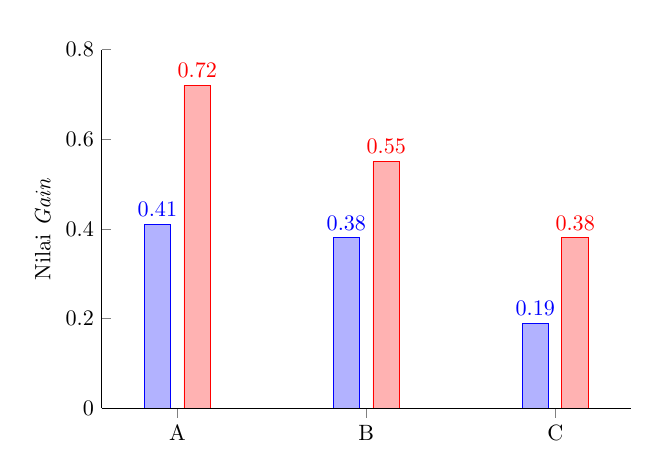
\begin{tikzpicture}[scale=0.8, transform shape]
\begin{axis}[
    every axis plot post/.style={/pgf/number format/fixed},
    ybar=6pt,
    bar width=12pt,
    x=3cm,
    ymin=0,
    axis on top,
    ylabel=Nilai \textit{Gain},
    ymax=0.8,
    xtick=data,
    enlarge x limits=0.2,
    symbolic x coords={A,B,C},
    restrict y to domain*=0:14, % Cut values off at 14
    visualization depends on=rawy\as\rawy, % Save the unclipped values
    after end axis/.code={ % Draw line indicating break
            \draw [ultra thick, white, decoration={snake, amplitude=1pt}, decorate] (rel axis cs:0,1.05) -- (rel axis cs:1,1.05);
        },
    nodes near coords={%
            \pgfmathprintnumber{\rawy}% Print unclipped values
        },
    axis lines*=left,
    clip=false
    ]
\addplot coordinates {(A,0.41) (B,0.38) (C,0.19)};
\addplot coordinates {(A,0.72) (B,0.55) (C,0.38)};
%\addplot coordinates {(A,6) (B,11) (C,7)};
\end{axis}
\end{tikzpicture}
%\includegraphics[width=0.6\textwidth]{Grafik1.pdf}
\caption{Peningkatan kemampuan pemecahan masalah untuk kelas kontrol (sebelah kiri, warna biru) dan kelas eksperimen (sebelah kanan, warna merah).
Ketrampilan yang dinilai adalah ketrampilan
(A) memahami masalah yang akan dipecahkan, (B) menyelidiki berbagai kemungkinan pemecahan masalah, dan
(C) mengevaluasi kualitas solusi pemecahan masalah.}
\label{Fig:Gain}
\end{figure}
\lipsum

\begin{figure}[htbp]
\centering
\begin{tikzpicture}
\begin{axis}
\addplot table [x=a, y=c, col sep=comma] {gambar/data.csv};
\end{axis}
\end{tikzpicture}
\caption{Ini adalah contoh grafik garis}
\end{figure}

\section{Contoh Lain}

Misalkan anda punya file:
\begin{verbatim}
\documentclass{article}

\usepackage{pgfplots}
\pgfplotsset{compat=newest}
\usetikzlibrary{calc}

\pagestyle{empty}
\usepackage{pgfplotstable}
\usepackage{mathpazo}
\usepackage[left=3.5cm, right=2cm,top=2.5cm, bottom=2cm]{geometry}
\usepackage{helvet}
\usepackage[eulergreek]{sansmath}
\pgfplotsset{
  tick label style = {font=\sansmath\sffamily},
  every axis label = {font=\sansmath\sffamily},
  legend style = {font=\sansmath\sffamily},
  label style = {font=\sansmath\sffamily}
}
\begin{document}

\input{250C}
\input{240C}

\end{document}
\end{verbatim}
Terlihat bahwa file di atas memanggil
file 250C.tex dan 240C.tex.
Isi dari file 250C.tex adalah
\begin{verbatim}
\pgfplotstableread
	{250C.csv}
	{\loadedtable}

\begin{tikzpicture}
	\begin{axis}[
	    %stack plots=y,
	    extra description/.code={\node  at  (0.8,0.85) 
                  {\bfseries (i) 250C};},
		ymin=0,
		xmax=9.5,
		minor tick num=4,
		enlarge x limits=false,
		axis on top,
		every axis plot post/.append style=
			{mark=none},
		const plot,
		xticklabels={,,},
		width=0.4\textwidth,
		height=0.3\textwidth,
%		ylabel= Load  (N),
		legend style={
			area legend,
			at={(0.5,-0.15)},
			anchor=north,
			legend columns=-1}]

%	\addplot[draw=blue,fill=blue!30!white]
	\addplot[draw=blue]
	 table[x=mm1,y=N1] from \loadedtable;
		%\closedcycle;
	\addplot table[x=mm2,y=N2] from \loadedtable;
	\addplot table[x=mm3,y=N3] 
		from \loadedtable;
	%\legend{1min load,nodes,cpus,processes}
	\end{axis}
	\pgfresetboundingbox
\useasboundingbox ($(current axis.south west)+(0,0.3ex)$)
    rectangle (current axis.north east);

\end{tikzpicture}
\end{verbatim}
Isi file 240C.tex adalah
\begin{verbatim}
\pgfplotstableread
	{240C.csv}
	{\loadedtable}

\begin{tikzpicture}
	\begin{axis}[
	    %stack plots=y,
	    extra description/.code={\node  at  (0.8,0.85) 
                  {\bfseries (ii) 240C};},
		ymin=0,
		xmax=9.5,
		minor tick num=4,
		enlarge x limits=false,
		axis on top,
		every axis plot post/.append style=
			{mark=none},
		const plot,
		xticklabels={,,},
		width=0.4\textwidth,
		height=0.3\textwidth,
%		ylabel= Load  (N),
		legend style={
			area legend,
			at={(0.5,-0.15)},
			anchor=north,
			legend columns=-1}]

%	\addplot[draw=blue,fill=blue!30!white]
	\addplot[draw=blue]
	 table[x=mm1,y=N1] from \loadedtable;
		%\closedcycle;
	\addplot table[x=mm2,y=N2] from \loadedtable;
	\addplot table[x=mm3,y=N3] 
		from \loadedtable;
	%\legend{1min load,nodes,cpus,processes}
	\end{axis}
	\pgfresetboundingbox
\useasboundingbox ($(current axis.south west)+(0,0.3ex)$)
    rectangle (current axis.north east);

\end{tikzpicture}
\end{verbatim}
Terlihat juga bahwa file 250C.tex memanggil
file 250C.csv, yang isinya kurang lebih (hanya 15 baris pertama
yang ditampilkan): 
\begin{verbatim}
No	mm1	N1	mm2	N2	mm3	N3
1	7.45E-009	30	7.45E-009	28	3.73E-009	26
2	0.02	34	0.02	36	0.02	36
3	0.03	40	0.03	36	0.03	46
4	0.05	44	0.06	52	0.05	56
5	0.07	46	0.07	58	0.06	56
6	0.09	48	0.08	58	0.08	68
7	0.1	50	0.1	70	0.1	72
8	0.12	48	0.12	72	0.12	74
9	0.13	48	0.13	72	0.14	76
10	0.15	46	0.17	76	0.15	78
11	0.17	48	0.19	78	0.17	80
12	0.18	48	0.2	80	0.18	80
13	0.2	50	0.22	82	0.2	84
14	0.22	54	0.24	86	0.22	96
15	0.23	58	0.25	90	0.24	104
\end{verbatim}
Hasilnya dapat dilihat pada Gambar~\ref{Fig:grafikTumpuk}.
\begin{figure}[htbp]
\includegraphics[width=\textwidth]{gambar/grafikTumpuk.png}
\caption{Tampilan grafik yang digabungkan secara vertikal.}
\label{Fig:grafikTumpuk}
\end{figure}

\section{Bar Graph dengan Error Bar}
\textit{Error bar} atau deviasi standar menunjukkan kualitas eksperimen.
Deviasi standar yang besar menunjukkan kualitas eksperimen yang buruk.
Namun demikian, deviasi standar tidak boleh dimanipulasi atau dimodifikasi
sehingga menjadi kecil.  Pengecilan deviasi semacam ini berbahaya karena
pada dasarnya kita tidak tahu nilai sebenarnya (yaitu nilai rata-rata) dari
eksperimen tersebut. Jika nilainya sudah diketahui, maka itu bukanlah penelitian
melainkan praktikum.

Contoh skrip \LaTeX untuk menghasilkan Gambar~\ref{Fig:bargraph-error}
adalah\footnote{Silahkan di modifikasi agar lebih menarik.}
\begin{verbatim}
      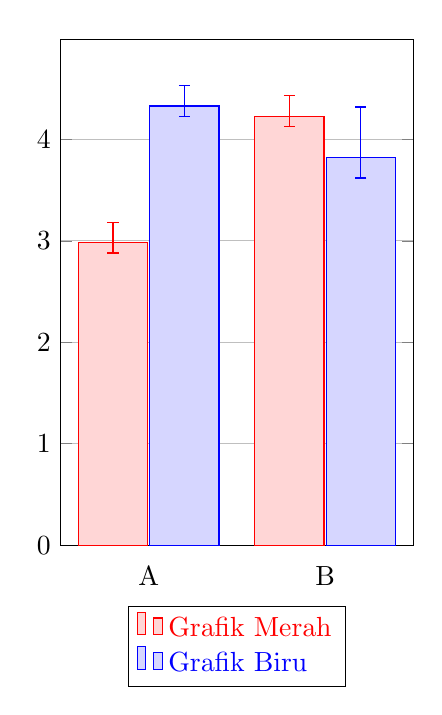
\begin{tikzpicture}
      \begin{axis}[
      width  = 0.50*\textwidth,
      height = 8cm,
      major x tick style = transparent,
      ybar=2*\pgflinewidth,
      bar width=25pt,
      ymajorgrids = true,
      symbolic x coords={A,B},
      xtick = data,
      scaled y ticks = false,
      enlarge x limits=0.50,
      ymin=0,
      legend cell align=left,
      legend style={at={(0.5,-0.12)},anchor=north},
  ]
      \addplot[red,style={fill=red!80!white!20},
error bars/.cd, y dir=both, y explicit]
          coordinates {
          (A, 2.98) += (0,0.2) -= (0,0.1)
          (B,4.23) += (0,0.2) -= (0,0.1)};

      \addplot[style={blue,fill=blue!80!white!20},
error bars/.cd, y dir=both, y explicit,error bar style=blue]
           coordinates {
           (A,4.33) += (0,0.2) -= (0,0.1)
           (B,3.82) += (0,0.5) -= (0,0.2)};

      \legend{\textcolor{red}{Grafik Merah}, \textcolor{blue}{Grafik Biru}}
  \end{axis}
  \end{tikzpicture}
\end{verbatim}
\begin{figure}[htbp]
        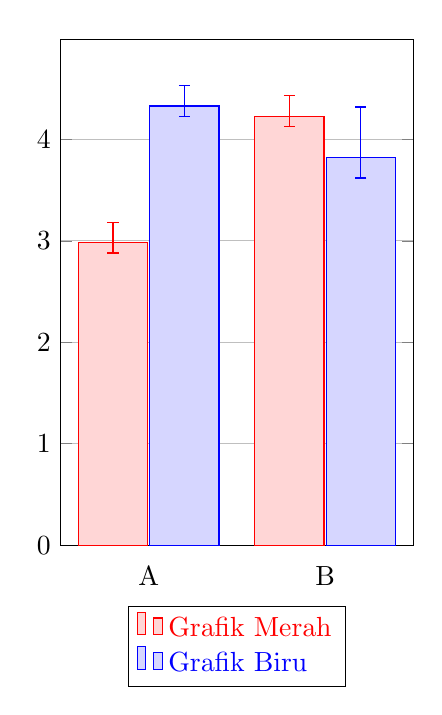
\begin{tikzpicture}
      \begin{axis}[
      width  = 0.50*\textwidth,
      height = 8cm,
      major x tick style = transparent,
      ybar=2*\pgflinewidth,
      bar width=25pt,
      ymajorgrids = true,
      symbolic x coords={A,B},
      xtick = data,
      scaled y ticks = false,
      enlarge x limits=0.50,
      ymin=0,
      legend cell align=left,
      legend style={at={(0.5,-0.12)},anchor=north},
  ]
      \addplot[red,style={fill=red!80!white!20},error bars/.cd, y dir=both, y explicit]
          coordinates {
          (A, 2.98) += (0,0.2) -= (0,0.1)
          (B,4.23) += (0,0.2) -= (0,0.1)};

      \addplot[style={blue,fill=blue!80!white!20},error bars/.cd, y dir=both, y explicit,error bar style=blue]
           coordinates {
           (A,4.33) += (0,0.2) -= (0,0.1)
           (B,3.82) += (0,0.5) -= (0,0.2)};

      \legend{\textcolor{red}{Grafik Merah}, \textcolor{blue}{Grafik Biru}}
  \end{axis}
  \end{tikzpicture}

  \caption{\textit{Bar-graph} berikut \textit{error bar}.}
  \label{Fig:bargraph-error}
\end{figure}

\chapter{Acuan}

Banyak style yang dapat digunakan untuk mengacu hasil penelitian 
yang telah dilakukan terdahulu.  Namun untuk skripsi 
di \institusiTulis, style yang digunakan adalah APA
(American Psychological Association).
Pemilihan style ini adalah karena APA sering digunakan 
dalam bidang pendidikan \autocite{styleGuide}.
Rincian style ini dapat dipelajari dari berbagai literatur,
termasuk yang ada di website \cite{APAPurdue}.
Usahakan untuk tidak mengacu website karena 
keberadaan website yang tidak jelas waktunya dan tidak memerlukan
adanya jaminan kualitas.

Tahapan penggunaan biblatex dengan style APA adalah sebagai berikut:
\begin{enumerate}
\item Pada preamble (di atas begin\{document\}) tuliskan:
\begin{Verbatim}[numbers=left,xleftmargin=5mm]
\usepackage[style=apa]{biblatex} 
\DeclareLanguageMapping{bahasai}{american-apa}

\addbibresource{example.bib} 
% nama file untuk daftar pustaka

\usepackage[autostyle=true]{csquotes} 
% perlu untuk kutipan bebas bahasa
\end{Verbatim}
Sebagai catatan, sebelumnya (melalui skripsiSTKIP.cls), telah 
dicantumkan 
\begin{Verbatim}[numbers=left,xleftmargin=5mm]
\usepackage[bahasai]{babel}
\end{Verbatim}
yang berguna untuk pemisahan suku kata sesuai dengan kaidah bahasa Indonesia.
\item Ditempat dimana daftar acuan akan dimunculkan,
tulislah:
\begin{Verbatim}[numbers=left,xleftmargin=5mm]
\printbibliography
\end{Verbatim}
\item File example.bib di atas, bisa mengandung:
\begin{Verbatim}[numbers=left,xleftmargin=5mm]
@article{Reference1,
	Abstract = {We have developed an enhanced Littrow configuration extended cavity diode laser (ECDL) that can be tuned without changing the direction of the output beam. The output of a conventional Littrow ECDL is reflected from a plane mirror fixed parallel to the tuning diffraction grating. Using a free-space Michelson wavemeter to measure the laser wavelength, we can tune the laser over a range greater than 10 nm without any alteration of alignment.},
	Author = {C. J. Hawthorn and K. P. Weber and R. E. Scholten},
	Journal = {Review of Scientific Instruments},
	Month = {12},
	Number = {12},
	Numpages = {3},
	Pages = {4477--4479},
	Title = {Littrow Configuration Tunable External Cavity Diode Laser with Fixed Direction Output Beam},
	Volume = {72},
	Url = {http://link.aip.org/link/?RSI/72/4477/1},
	Year = {2001}}

@article{Reference3,
	Abstract = {Operating a laser diode in an extended cavity which provides frequency-selective feedback is a very effective method of reducing the laser's linewidth and improving its tunability. We have developed an extremely simple laser of this type, built from inexpensive commercial components with only a few minor modifications. A 780~nm laser built to this design has an output power of 80~mW, a linewidth of 350~kHz, and it has been continuously locked to a Doppler-free rubidium transition for several days.},
	Author = {A. S. Arnold and J. S. Wilson and M. G. Boshier and J. Smith},
	Journal = {Review of Scientific Instruments},
	Month = {3},
	Number = {3},
	Numpages = {4},
	Pages = {1236--1239},
	Title = {A Simple Extended-Cavity Diode Laser},
	Volume = {69},
	Url = {http://link.aip.org/link/?RSI/69/1236/1},
	Year = {1998}}

@article{Reference2,
	Abstract = {We present a review of the use of diode lasers in atomic physics with an extensive list of references. We discuss the relevant characteristics of diode lasers and explain how to purchase and use them. We also review the various techniques that have been used to control and narrow the spectral outputs of diode lasers. Finally we present a number of examples illustrating the use of diode lasers in atomic physics experiments. Review of Scientific Instruments is copyrighted by The American Institute of Physics.},
	Author = {Carl E. Wieman and Leo Hollberg},
	Journal = {Review of Scientific Instruments},
	Keywords = {Diode Laser},
	Month = {1},
	Number = {1},
	Numpages = {20},
	Pages = {1--20},
	Title = {Using Diode Lasers for Atomic Physics},
	Volume = {62},
	Url = {http://link.aip.org/link/?RSI/62/1/1},
	Year = {1991}}

@online{styleGuide,
author = {University Library, American University},
title = {Which style should I use ?},
Url = {http://subjectguides.library.american.edu/c.php?g=175008&p=1154150},
urldate = {2016-01-03}
}

@online{APAPurdue,
title = {Purdue Online Writing Lab},
Url = {https://owl.english.purdue.edu/owl/resource/560/1/},
urldate = {2016-01-03}
}
\end{Verbatim}

\item Cara menggunakan / memanggil acuan adalah dengan menggunakan 
autocite, misalnya:
\begin{Verbatim}[numbers=left,xleftmargin=5mm]
Rincian style ini dapat dipelajari dari berbagai literatur,
termasuk yang ada di website \autocite{APAPurdue}.
\end{Verbatim}
\end{enumerate}

\section{Cara mengacu dengan biber/biblatex}
Yang paling sering diperlukan, paling tidak ada 2, yaitu:
\begin{enumerate}
\item Dengan menuliskan
\begin{Verbatim}[numbers=left,xleftmargin=5mm]
bla bla\autocite{Reference1,Reference2,Reference3}
\end{Verbatim}
akan diperoleh teks 
bla bla\autocite{Reference1,Reference2,Reference3}.
\item Dengan menuliskan
\begin{Verbatim}[numbers=left,xleftmargin=5mm]
seperti dibahas oleh 
\textcite{Reference1,Reference2,Reference3}.
\end{Verbatim}
akan diperoleh teks
seperti dibahas oleh \textcite{Reference1,Reference2,Reference3}.
\end{enumerate}

\section{Cara kompile acuan}
Ada 4 jurus, yaitu:
\begin{enumerate}
\item \texttt{xelatex skripsi}
\item \texttt{biber skripsi}
\item \texttt{xelatex skripsi}
\item \texttt{xelatex skripsi}
\end{enumerate}
Beberapa penjelasannya adalah
\begin{enumerate}
\item Tulisan \texttt{skripsi} di atas adalah 
nama file berakhiran \texttt{tex} yang akan 
di \textit{typeset} dengan \LaTeX.
\item Walau file bibliography yang berakhiran 
\texttt{bib} bernama file \texttt{example.bib},
pernyataan \texttt{biber} tetap mengacu ke nama file
yang memanggil \texttt{example.bib} (dalam hal ini file 
\texttt{skripsi} 
di atas).  
\item Setelah pernyataan \texttt{biber skripsi} di atas,
harus dilakukan dua kali \texttt{xelatex skripsi},
karena 
\begin{enumerate}
\item tahap pertama adalah penulisan ke file berakhiran
\texttt{bbl}
\item tahap kedua adalah penulisan ke file pdf.
\end{enumerate}
\end{enumerate}



\appendix % Cue to tell LaTeX that the following "chapters" are Appendices

% Include the appendices of the thesis as separate files from the Appendices folder
% Uncomment the lines as you write the Appendices

\include{Appendices/AppendixA}
%\include{Appendices/AppendixB}
%\include{Appendices/AppendixC}

%----------------------------------------------------------------------------------------
%	BIBLIOGRAPHY
%----------------------------------------------------------------------------------------

\printbibliography[heading=bibintoc]

%----------------------------------------------------------------------------------------

\end{document}  
